% Kozierok, ch. 18
\chapter{IP subnet addressing (subnetting) concepts}
\label{chap:kozierok-ch18}

In the previous chapter, we looked at the original classful IP
addressing scheme, which conceptually divides a large internetwork into
a simple two-level hierarchy that includes many {\emph{networks}} of
different sizes, each of which contains a number of {\emph{hosts}}. The
system works well for smaller organizations that may connect all their
machines in a single network. However, it lacks flexibility for large
organizations that often have many subnetworks, or {\emph{subnets}}. To
better meet the administrative and technical requirements of larger
organizations, the classful IP addressing system was enhanced through a
technique known as {\emph{subnet addressing}}, or more simply,
{\emph{subnetting}}.

In this chapter, I describe the concepts and general techniques
associated with IP subnet addressing. I begin with an overview of
subnetting, including a discussion of the motivation for the system and
its advantages. I discuss how the traditional two-level method for
dividing IP addresses becomes three-level for subnetting. I talk about
subnet masks and how they are used in calculations for addressing and
routing. I discuss the default subnet masks used to represent the
classful class A, B, and C networks in a subnetting environment and then
how custom subnet masks are used for these classes.
I then discuss subnet identifiers and general concepts behind determining subnet and host addresses in a subnet environment.
I provide summary tables for subnetting class A, B, and C networks.
I conclude with a brief discussion of \emph{variable-length subnet masking} (VLSM), an enhancement of conventional subnetting that improves its flexibility further.

\begin{note}
I provide a great deal of coverage of subnetting, because
understanding it is an important part of learning about how IP addresses
work, and hence, how TCP/IP functions. However, the technique is today
considered mostly historical because it is based on classful
addressing. The concept of a subnet and subnet mask has certainly not
disappeared, but the idea of being assigned a class A, B, or C Internet
address block and then explicitly subnetting it is no longer relevant.
\end{note}


\begin{note}
This is the first of two chapters dedicated to IP address subnetting.
\Vref{chap:kozierok-ch19} describes the step-by-step process for subnetting using examples.
If you find that after reading this concepts section that you don't quite understand subnetting,
try reading the example-based section, and you may find that it helps make it all click.
On the other hand, if you are already somewhat familiar with subnetting, you may find that you can skip this concepts section
and just go through the step-by-step examples.
You will find much more in that chapter in the way of gory details of subnet mask, subnet
address, and host address calculations.
Putting the practical details there allows this section to concentrate on concepts without getting too
bogged down in numbers.
\end{note}


\begin{backgroundinfo}
Understanding subnetting requires familiarity with binary numbers and how they are manipulated.
This includes the concept of using boolean operators such as AND to ``mask'' binary digits.
If reading that last sentence made you go ``huh?'' I strongly recommend reviewing the background section on
computing mathematics (\vref{chap:binary-numbers}) before you proceed.
\end{backgroundinfo}




\section{IP subnet addressing overview, motivation, and advantages}

As I discussed in the previous chapter, IP addressing was originally
designed around the assumption of a strict two-level hierarchy for internetworks: the first level was the network, and the second level the
host.
Each organization was usually represented by a single network identifier (network ID) that indicated a class A, B, or C block
dedicated to them.
Within that network, the organization needed to put all of the devices it wanted to connect to the public IP network.

It did not take long after this scheme was developed for serious
inadequacies in it to be noticed, especially by larger organizations. In
order to address this problem, RFC 950 {[}1985{]} defined a new
addressing procedure called {\emph{subnet addressing}} or
{\emph{subnetting}}.

Subnet addressing adds an additional hierarchical level to the way IP
addresses are interpreted: Instead of having just hosts, the network has
{\emph{subnets}} and hosts. Each subnet is a subnetwork, and functions
much the way a full network does in conventional classful addressing. A
three-level hierarchy is thus created: networks, which contain subnets,
each of which then has a number of hosts. Thus, an organization can
organize hosts into subnets that reflect the way internal networks are
structured. In essence, subnet addressing allows each organization to
have its own internetwork within the Internet. This change brought
numerous advantages over the old system, such as the following:
\begin{description}
   \item[Better match to physical network structure]
      Hosts can be grouped into subnets that reflect the way they are actually structured in the organization's physical network.

   \item[Flexibility]
      The number of subnets and number of hosts per subnet can be customized for each organization.
      Each can decide on its own subnet structure and change it as required.

   \item[Invisibility to public Internet]
      Subnetting was implemented so that the internal division of a network into subnets is visible only within the organization.
      To the rest of the Internet, the organization is still just one big, flat network.
      This also means that any changes made to the internal structure are not visible outside the organization.

   \item[No need to request new IP addresses]
      Organizations don't need to constantly requisition more IP addresses, as they would in the workaround of using multiple small class C blocks.

   \item[No routing table entry proliferation]
      Since the subnet structure exists only within the organization, routers outside that organization know nothing about it.
      The organization still maintains a single (or perhaps a few) routing table entries for all of its devices.
      Only routers inside the organization need to worry about routing between subnets.
\end{description}


The change to subnetting affects both addressing and routing in IP
networks. Addressing changes because, instead of having just a network
ID and host ID, you now also have a {\emph{subnet ID}} to be concerned
with. The size of the subnet ID can vary for each network, so an
additional piece of information is needed to supplement the IP address
to indicate what part of the address is the subnet ID and what part is
the host ID. This is a 32-bit number commonly called a {\emph{subnet
mask}}. The mask is used both for calculating subnet and host addresses,
and by routers for determining how to move IP datagrams around a
subnetted network.

Routing changes because of the additional level of hierarchy. In regular
classful addressing, when a router receives an IP datagram, it only
needs to decide if the destination is on the same network or a different
network. Under subnetting, it must also look at the subnet ID of the
destination and make one of three choices: same subnet, different subnet
on the same network, or different network. Changes are also required to
routing protocols, such as the Routing Information Protocol (RIP; see
\protect\hyperlink{ch38.html}{Chapter~38}), to deal with subnets and
subnet masks.


\begin{keyconcept}
Subnet addressing adds an additional hierarchical level to how IP addresses are interpreted by dividing an organization's IP network into subnets.
This allows each organization to structure its address space to match its internal physical networks, rather than being forced to treat them a flat block.
This solves a number of problems with the original classful addressing scheme, but requires changes to how addressing and routing work, as well as modifications to several TCP/IP protocols.
\end{keyconcept}

It's funny, but the main drawbacks to subnetting, compared with the
older addressing scheme, have more to do with understanding how
subnetting works than with the technology itself. More effort is
required to deal with addressing and routing in a subnet environment,
and administrators must learn how to subdivide their network into
subnets and properly assign addresses. This can be a bit confusing to
someone who is new to subnetting. However, the technology today is quite
well established, so even this is not much of a problem.


\section{IP subnetting: three-level hierarchical IP subnet addressing}

As I mentioned earlier, subnetting adds an additional level to the hierarchy
of structures used in IP addressing. To support this, IP addresses must
be broken into three elements instead of two. This is done by leaving
the network ID alone and dividing the host ID into a subnet ID and host
ID. These subnet ID bits are used to identify each subnet within the
network. Hosts are assigned to the subnets in whatever manner makes the
most sense for that network.

Interestingly, the earlier analogy to telephone numbers still holds in
the world of subnetting and shows how subnetting changes the way IP
addresses are interpreted. For example, a phone number like (401)
555-7777 has an area code (401) and a local number (555-7777). The local
number, however, can itself be broken down into two parts: the exchange
(555) and the local extension (7777). This means phone numbers really
are comprised of three hierarchical components, just as IP addresses are
in subnetting.

Of course, the number of bits in an IP address is fixed at 32.
This means that in splitting the host ID into subnet ID and host ID, you reduce the size of the host ID portion of the address.
In essence, you are stealing bits from the host ID to use for the subnet ID.
Class~A networks have 24 bits to split between the subnet ID and host ID; class B networks have 16; and class C networks have only 8.


\begin{keyconcept}
A classful network is subnetted by dividing its
host ID portion, leaving some of the bits for the host ID while
allocating others to a new subnet ID. These bits are then used to
identify individual subnets within the network, into which hosts are
assigned.
\end{keyconcept}

Now remember that when we looked at the sizes of each of the main
classes in the previous chapter, we saw that, for each class, the number
of networks and the number of hosts per network are a function of how
many bits we use for each. The same applies to the splitting of the host
ID. Since we are dealing with binary numbers, the number of subnets is
two to the power of the size of the subnet ID field. Similarly, the
number of hosts per subnet is two to the power of the size of the host
ID field (less two for excluded special cases).

Let's take a brief example to see how this works. Imagine that you start
with class B network 154.71.0.0, with 16 bits for the network ID
(154.71) and 16 are for the host ID. In regular classful addressing,
there are no subnets and 65,534 hosts total. To subnet this network, you
can decide to split those 16 bits however you feel best suits the needs
of the network: 1 bit for the subnet ID and 15 for the host ID, or 2 and
14, 3 and 13, and so on. Most any combination will work, as long as the total is 16;
I've used 5 and 11 in the example shown in \cref{fig:subnetting-class-b-example}.
The more bits you steal from the host ID for the subnet ID, the more subnets you can have, but the fewer hosts you can have for each subnet.


\begin{figure}
   \centering
   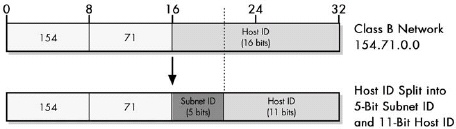
\includegraphics[width=.7\textwidth]{images/subnetting-class-b-example.jpg}
   \caption
      [Subnetting a class B network]
      {Subnetting a class B network -- We begin with the class B network 154.71.0.0, which has 16 bits in its host ID block.
      We then subnet this network by dividing the host ID into a subnet ID and host ID.
      In this case, 5 bits have been allocated to the subnet ID, leaving 11 bits for the host ID.}
   \label{fig:subnetting-class-b-example}
\end{figure}


Choosing how to split the host ID into subnet and host bits is one of
the most important design considerations in setting up a subnetted IP
network. The number of subnets is generally determined based on the
number of physical subnetworks in the overall organizational network,
and the number of hosts per subnetwork must not exceed the maximum
allowed for the particular subnetting choice you make. Choosing how to
divide the original host ID bits into subnet ID bits and host ID bits is
sometimes called {\emph{custom subnetting}} and is described in more
detail later in this chapter.



\section{IP subnet masks, notation, and subnet calculations}

Subnetting divides an organization's network into a two-level structure of subnets
and hosts that is entirely internal and hidden from all other
organizations on the Internet. One of the many advantages of this is
that each organization gets to make its own choice about how to divide
the classful host ID into subnet ID and host ID.

In a nonsubnetted classful environment, routers use the first octet of
the IP address to determine what the class of the address is, and from
this they know which bits are the network ID and which are the host ID.
When you use subnetting, these routers also need to know how that host
ID is divided into subnet ID and host ID. However, this division can be
arbitrary for each network. Furthermore, there is no way to tell how
many bits belong to each simply by looking at the IP address.

In a subnetting environment, the additional information about which bits
are for the subnet ID and which are for the host ID must be communicated
to devices that interpret IP addresses. This information is given in the
form of a 32-bit binary number called a {\emph{subnet mask}}. The term
{\emph{mask}} comes from the binary mathematics concept called
{\emph{bit
masking}}. This is a technique where a special pattern of ones and zeros
can be used in combination with boolean functions such as AND and OR to
select or clear certain bits in a number. (I explain bit masking in the
background section on binary numbers and mathematics, in \vref{chap:binary}.)



\subsection{Function of the subnet mask}

There's something about subnet masks that seems to set people's hair on end, especially if they aren't that familiar with binary numbers.
However, the idea behind them is quite straightforward.
The mask is a 32-bit number, just as the IP address is a 32-bit number.
Each of the 32 bits in the subnet mask corresponds to the bit in the IP address in the same location in the number.
The bits of the mask in any given subnetted network are chosen so that the bits used for either the network ID or subnet ID are ones,
while the bits used for the host ID are zeros.


\begin{keyconcept}
The \emph{subnet mask} is a 32-bit binary number that accompanies an IP address.
It is created so that it has a one bit for each corresponding bit of the IP address that is part of its
network ID or subnet ID, and a zero for each bit of the IP address's
host ID. The mask thus tells TCP/IP devices which bits in that IP
address belong to the network ID and subnet ID, and which are part of the host ID.
\end{keyconcept}

Why bother doing this with a 32-bit binary number? The answer is the
magic of boolean logic. You use the subnet mask by applying the boolean
AND function between it and the IP address. For each of the 32 ``bit
pairs'' in the IP address and subnet mask, you employ the AND function,
the output of which is one only if both bits are one. What this means in
practical terms is the following, for each of the 32 bits:

\begin{description}
   \item[Subnet mask bit is a one]
      In this case, you are ANDing either a zero or one in the IP address with a one.
      If the IP address bit is a zero, the result of the AND will be zero; if it is a one, the AND will be one.
      In other words, \emph{where the subnet bit is a one, the IP address is preserved unchanged}.

   \item[Subnet mask bit is a zero]
      Here, you are ANDing with a zero, so the result is always zero, regardless of what the IP address is.
      Thus, \emph{when the subnet bit is a zero, the IP address bit is always cleared to zero}.
\end{description}

Thus, when you use the subnet mask on an IP address, the bits in the
network ID and subnet ID are left intact, while the host ID bits are
removed. Like a mask that blocks part of your face but lets other parts
show, the subnet mask blocks some of the address bits (the host bits)
and leaves others alone (the network and subnet bits). A router that
performs this function is left with the address of the subnet. Since it
knows from the class of the network what part is the network ID, it also
knows what subnet the address is on.


\begin{keyconcept}
To use a subnet mask, a device performs a boolean AND operation between each bit of the subnet mask and each corresponding bit of an IP address.
The resulting 32-bit number contains only the network ID and subnet ID of the address, with the host ID cleared to zero.
\end{keyconcept}


\subsection{Subnet mask notation}

Like IP addresses, subnet masks are always used as a 32-bit binary number by computers.
And like IP addresses, using them as 32-bit binary numbers is difficult for humans.
Therefore, they are usually converted to dotted decimal notation for convenience, just as IP addresses are.

For example, suppose you decide to subnet the class B network 154.71.0.0 using 5 bits for the subnet ID and 11 bits for the host ID (see \cref{fig:determining-subnet-mask}).
In this case, the subnet mask will have 16 ones for the network portion
(since this is class B) followed by 5 ones for the subnet ID, and 11
zeros for the host ID. That's 11111111 11111111 {\textbf{11111}}000
00000000 in binary, with the bits corresponding to the subnet ID
highlighted. In dotted decimal, the subnet mask would be 255.255.248.0.


\begin{figure}
   \centering
   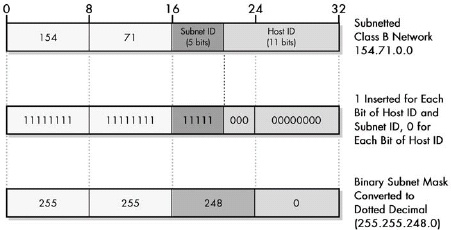
\includegraphics[width=.7\textwidth]{images/determining-subnet-mask.jpg}
   \caption
      [Determining the subnet mask of a subnetted network]
      {Determining the subnet mask of a subnetted network -- The class B network from \vref{fig:subnetting-class-b-example} is shown at the top,
      with 5 bits assigned to the subnet ID and 11 bits left for the host ID.
      To create the subnet mask, you fill in a 32-bit number with 1 for each network ID and subnet ID bit, and 0 for each host ID bit.
      You can then convert this to dotted decimal.}
   \label{fig:determining-subnet-mask}
\end{figure}



\subsection{Applying the subnet mask: an example}

Now, let's see how the subnet mask might be used. Suppose you have a
host on this network with an IP of 154.71.150.42 and a router needs to
figure out which subnet this address is on.
To do so, it performs the masking operation shown in \cref{tab:determining-prefix}
and
\protect\hyperlink{ch18s03.htmlux5cux23determining_the_subnet_id_of_an_ip-id001}{Figure~18-3}.

\begin{table}
   \centering
   \begin{tabular}{rllll}
   \textit{component}   & octet 1   & octet 2   & octet 3                     & octet 4   \\[1ex]
   \textit{IP address}  & 1001 1010 & 0100 0111 & 1001 0110                   & 0010 1010 \\
   \textit{subnet mask} & 1111 1111 & 1111 1111 & \textbf{1111} \textbf{1}000 & 0000 0000 \\
   \textit{AND masking} & 1001 1010 & 0100 0111 & \textbf{1001} \textbf{0}000 & 0000 0000 \\
   \end{tabular}
   \caption{Determining the subnet ID of an IP adress through subnet masking}
   \label{tab:determining-prefix}
\end{table}


\begin{figure}
   \centering
   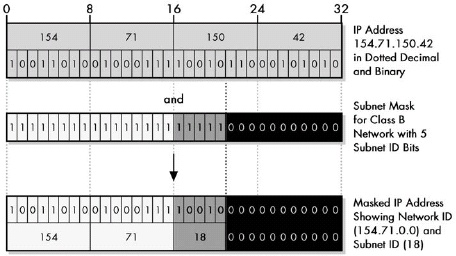
\includegraphics[width=.7\textwidth]{images/determining-prefix.jpg}
   \caption
      [Determining the subnet ID of an IP address through subnet masking]
      {Determining the subnet ID of an IP address through subnet masking -- Subnet masking involves performing a boolean AND between each
      corresponding bit in the subnet mask and the IP address.
      The subnet mask can be likened to a physical mask; each 1 in it lets the corresponding bit of the IP address show through, while each 0 blocks the
      corresponding IP address bit.
      In this way the host ID bits of the address are stripped so the device can determine the subnet to which the address belongs.}
   \label{fig:determining-prefix}
\end{figure}


This result, 154.71.144.0, is the IP address of the subnet to which 154.71.150.42 belongs.
There is no need to explicitly differentiate the network ID bits from the subnet ID bits, because you are still using classful addresses.
Any router can see that since the first two bits of the address are 10, this is a class B address.
So the network ID is 16 bits, and this means the subnet ID must be bits 17 to 21, counting from the left.
Here, the subnet is the portion highlighted earlier: 10010, or subnet 18.
(I'll explain this better in \vref{sec:ip-custom-subnet-masks}.)


\begin{keyconcept}
The subnet mask is often expressed in dotted decimal notation for convenience, but is used by computers as a binary
number and usually must be expressed in binary to understand how the mask works and the number of subnet ID bits it represents.
\end{keyconcept}


\subsection{Rationale for subnet mask notation}

In practical terms, the subnet mask actually conveys only a single piece
of information: the line between the subnet ID and host ID. Then why
bother with a big 32-bit binary number in that case, instead of just
specifying the bit number where the division occurs? Instead of carrying
the subnet mask of 255.255.248.0 around, why not just divide the IP
address after bit 21? Even if devices want to perform a masking
operation, couldn't they just create the mask as needed?

That's a very good question. There are two historical reasons:
efficiency considerations and support for
noncontiguous
masks. The subnet mask expression is efficient because it allows routers
to perform a quick masking operation to determine the subnet address.
(This is not really an issue today given the speed of today's machines.)

When splitting the bits in the host ID for subnet ID and host ID, RFC
950 specifies that they may be split in more than one place. In the
previous example, you could, instead of splitting the 16 bits into 5
bits for subnet ID and 11 for host ID, have done it as 2 bits for the
subnet ID, then 4 bits for the host ID, then 3 more bits for the subnet
ID, and finally 7 more bits for host ID. This would be represented by
the subnet mask pattern 11000011 10000000 for those 16 bits (following
the 16 ones for the network ID). Of course, subnetting this way makes
assigning addresses \emph{extremely} confusing.
For this reason, while technically legal, noncontiguous subnet masking is not recommended and not done in practice.

Given that noncontiguous masks are not used, and today's computers are
faster, the alternative method of expressing masks with just a single
number is now often used. Instead of writing
``IP address of 154.71.150.42 with subnet mask of 255.255.248.0,'' you can simply
write ``154.71.150.42\textbf{/21}.''
This is sometimes called \emph{slash notation} or \emph{classless inter-domain routing} (CIDR) notation.
While this is more commonly used in variable-length subnet masking (VLSM) environments and is the standard for specifying classless addresses under the CIDR addressing scheme (see \vref{chap:kozierok-ch20}), it is also sometimes seen in regular subnetting discussions.

\begin{note}
Since these weird masks were never really used, some resources
say that the subnet mask always had to be contiguous, but this is not true -- originally, it was legal but advised against.
Later, this practice became so out of favor that many hardware devices would not support it.
Today, now that classless addressing and CIDR are standard, noncontiguous masks are simply illegal.
\end{note}




\section{IP default subnet masks for address classes A, B, and C}

In order to better understand how subnets divide a class A, B, or C network, let's
look at how the class A, B, and C networks are represented in a
subnetted environment. This might seem unnecessary if you aren't
planning to create subnets, but the fact is, once subnetting became
popular, most operating systems, networking hardware, and software
assumed that subnetting would be used. Even if you decide not to subnet,
you may need to express your unsubnetted network using a subnet mask.

In essence, a nonsubnetted class A, B, or C network can be considered
the default for the more general, custom-subnetted network. You can
think of a nonsubnetted network as being the case where you choose to
divide the host ID so that exactly zero bits are used for the subnet ID,
and all the bits are used for the host ID. This default case is the
basis for the more practical subnetting you will examine shortly.

As is always the case, the subnet mask for a default, unsubnetted Class
A, B, or C network has ones for each bit that is used for the network ID
or subnet ID and zeros for the host ID bits. Of course, I just said you
aren't subnetting, so there {\emph{are}} no subnet ID bits! Thus, the
subnet mask for this default case has ones for the network ID portion
and zeros for the host ID portion. This is called the {\emph{default
subnet mask}} for each of the IP address classes.

Since class A, B, and C divide the network ID from the host ID on octet
boundaries, the subnet mask will always have all ones or all zeros in an
octet. Therefore, the default subnet masks will always have 255s or 0s
when expressed in decimal notation.
\Cref{tab:default-subnet-masks} summarizes the default subnet masks for each of the classes.
They are also shown graphically in \cref{fig:default-subnet-masks}.


\begin{table}
   \centering
   \begin{tabular}{rlrrrr}
   \textit{class} & NID/HID & octet 1 & octet 2 & octet 3 & octet 4 \\[1ex]
   \textit{A}     & 8/24    & 255     & 0       & 0       & 0       \\
   \textit{B}     & 16/16   & 255     & 255     & 0       & 0       \\
   \textit{C}     & 24/8    & 255     & 255     & 255     & 0       \\
   \end{tabular}
   \caption{Default subnet masks for class A, class B, and class C networks}
   \label{tab:default-subnet-masks}
\end{table}


\begin{figure}
   \centering
   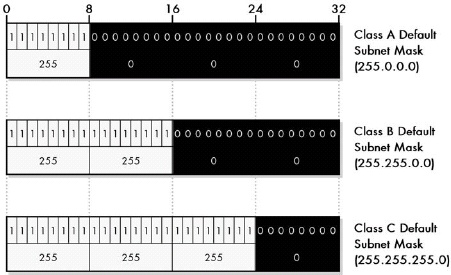
\includegraphics[width=.7\textwidth]{images/default-subnet-masks.jpg}
   \caption{Default subnet masks for class A, class B, and class C networks}
   \label{fig:default-subnet-masks}
\end{figure}

Thus, the three default subnet masks are 255.0.0.0 for class A, 255.255.0.0 for class B, and 255.255.255.0 for class C.

While all default subnet masks use only 255 and 0, not all subnet masks with 255 and 0 are defaults.
There are a small number of custom subnets that divide on octet boundaries as well. These are as follows:

\begin{description}
   \item[255.255.0.0]
      This is the default mask for class B, but can also be the custom subnet mask for dividing a class A network using 8~bits for the subnet ID
      (leaving 16~bits for the host ID).

   \item[255.255.255.0]
      This is the default subnet mask for class C, but can be a custom class A with 16 bits for the subnet ID \emph{or} a class B with 8 bits for the subnet ID.
\end{description}


\begin{keyconcept}
Each of the three IP unicast and broadcast address classes, A, B, and C, has a \emph{default subnet mask} defined
that has a one for each bit of the class's network ID, a zero for each bit of its host ID, and no subnet ID bits.
The three default subnet masks are 255.0.0.0 for class A, 255.255.0.0 for class B, and 255.255.255.0 for class C.
\end{keyconcept}




\section{IP custom subnet masks}
\label{sec:ip-custom-subnet-masks}

A default subnet mask doesn't really represent subnetting because you
are assigning zero bits to the subnet ID. To do real subnetting, you
must dedicate at least one of the bits of the presubnetted host ID to
the subnet ID.

Since you can choose the dividing point between subnet ID and host ID to suit the network, this is sometimes called \emph{customized subnetting}.
The subnet mask that you use when creating a customized subnet is, in turn, called a \emph{custom subnet mask}.
The custom subnet mask is used by network hardware to determine how you have decided to divide the subnet ID from the host ID in the network.



\subsection{Deciding how many subnet bits to use}

The key decision in customized subnetting is how many bits to take from
the host ID portion of the IP address to put into the subnet ID.
You'll recall that the number of subnets
possible on the network is two to the power of the number of bits you
use to express the subnet ID, and the number of hosts possible per
subnet is two to the power of the number of bits left in the host ID
(less two, as I explain later in this section).

Thus, the decision of how many bits to use for each of the subnet ID and
host ID represents a fundamental trade-off in subnet addressing:

\begin{itemize}
\item
  Each bit taken from the host ID for the subnet ID doubles the number
  of subnets that are possible in the network.
\item
  Each bit taken from the host ID for the subnet ID (approximately)
  halves the number of hosts that are possible within each subnet on the
  network.
\end{itemize}

For example, say you start with a class B network with the network
address 154.71.0.0. Since this is class B, 16 bits are for the network
ID (154.71) and 16 are for the host ID. In the default case, there are
no subnets and 65,534 hosts total. To subnet this network, you can use
the following:

\begin{itemize}
   \item
      One bit for the subnet ID and 15 bits for the host ID. If you do this,
      then the total number of subnets is $2^{1} = 2$.
      The first subnet is 0, and the second is 1.
      The number of hosts available  for each subnet is $2^{15}-2$, or 32766.
   \item
      Two bits for the subnet ID and 14 for the host ID.
      In this case, you double the number of subnets.
      You now have $2^{2}= 4$ subnets: 00, 01, 10, and 11 (subnets 0, 1, 2, and 3).
      But the number of hosts is now only $2^{14}-2$, or 16382.
   \item
      Any combination of bits that add up to 16 as long as they allow you at least two hosts per subnet: 4 and 12, 5 and 11, and so on.
\end{itemize}

The way you decide to divide the classful host ID into subnet ID and
host ID bits is the key design decision in subnetting. You make your
choice based on the number of subnets in the network, and also on the
maximum number of hosts that need to be assigned to each subnet in the
network. For example, if you have 10 total subnets for your class B
network, you need 4 bits to represent this, because 2\textsuperscript{4}
is 16 while 2\textsuperscript{3} is only 8. This leaves 12 bits for the
host ID, for a maximum of 4,094 hosts per subnet.

However, suppose instead that you have 20 subnets. If so, 4 bits for
subnet ID won't suffice; you need 5 bits ($2^{5}=32$).
This means that you now have only 11 bits for the host ID, for a maximum of 2,046 hosts per subnet.
(Step 2 of the practical subnetting example in \vref{chap:kozierok-ch19} discusses these decisions in more detail.)

Now if you have 20 subnets and also need a maximum of 3,000 hosts per
subnet, you have a problem. You need 5 bits to express 20 different
subnets, but you need 12 bits to express the number 3,000 for the host
ID. That's 17 bits -- one too many. What's the solution? You might be able to
shuffle your physical networks so that you only have 16. If not, you
need a second class B network.

\begin{keyconcept}
The fundamental trade-off in subnetting is that each addition of a bit to the subnet ID (and thus, subtraction of that bit from the host ID)
doubles the number of subnets, and approximately halves the number of hosts in each subnet.
Each subtraction of a bit from the subnet ID (and addition of that bit to the host ID) does the opposite.
\end{keyconcept}


\subsection{Determining the custom subnet mask}

Once you determine how many bits to devote to the subnet and host IDs,
you can determine the subnet mask. You begin with the default subnet
mask in binary for the appropriate class of the network. You start with
the leftmost zero in that mask and change as many bits to one as you
have dedicated to the subnet ID, at which point you can express the subnet mask in dotted decimal form.
\Cref{fig:custom-subnet-masks} shows how the custom subnet mask can be determined for each of the
subnetting options of a class C network in both binary and decimal.

Consider the class C network 200.13.94.0 in \cref{fig:custom-subnet-masks}.
There are eight bits in the original host ID, which gives you six different subnetting options
(you can't use seven or eight bits for the subnet ID, for reasons I will discuss shortly).%
   \footnote{A prefix-length of 31 is allowed on point-to-point links and has been for five years when \cite{kozierok05} got published. See RFC~3021 for details.}
Suppose you use three of these for the subnet ID, leaving five for the host ID.
To determine the custom subnet mask, you start with the class C default subnet mask:

\begin{quote}
1111 1111\quad 1111 1111\quad 1111 1111\quad 0000 0000
\end{quote}

You then change the first three zeros to ones, to get the custom subnet mask:

\begin{quote}
1111 1111\quad 1111 1111\quad 1111 1111\quad \textbf{111}0 0000
\end{quote}
In dotted decimal format, this is 255.255.255.224.


\begin{note}
Once you've made the choice of how to subnet, you determine the custom subnet mask by starting with
the default subnet mask for the network and changing each subnet ID bit from a zero to a one.
\end{note}

\begin{note}
In regular subnetting, the choice of how many bits to use for the subnet ID is fixed for the entire network.
You can't have subnets of different sizes -- they must all be the same.
Thus, the number of hosts in the largest subnet will dictate how many bits you need for the host ID.
This means that in the previous case, if you had a strange configuration where 19 subnets had only 100 hosts each but the 20th had 3,000, you would have a problem.
If this were the case, you could solve the problem easily by dividing that one oversized subnet into two or more smaller ones.
An enhancement to subnetting called variable-length subnet masking (VLSM) was created in large part to remove this restriction.
VLSM is described later in the chapter.
\end{note}


\begin{figure}
   \centering
   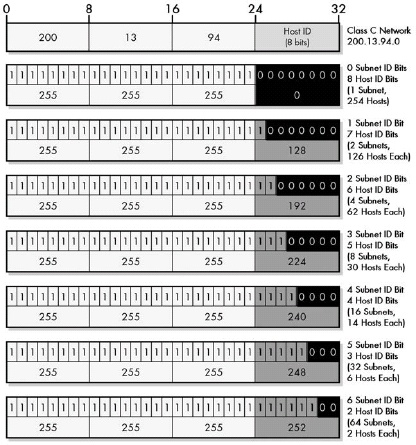
\includegraphics[width=\textwidth]{images/custom-subnet-masks.jpg}
   \caption
      [Custom subnet masks for class C networks]
      {Custom subnet masks for class C networks --
      Since there are host ID bits in a class C network address, there are six different ways that the network can be subnetted.
      Each corresponds to a different custom subnet mask, which is created by changing the allocated subnet ID bits from zero to one.}
   \label{fig:custom-subnet-masks}
\end{figure}



\subsection{Subtracting two from the number of hosts per subnet and (possibly) subnets per network}

You've seen how you must subtract two from the number of hosts allowed
in each network in regular classful addressing. This is necessary
because two host IDs in each subnet have special meanings: the all-zeros
host ID (for ``this network'') and the all-ones host ID (for broadcasts to
all hosts on the network). These restrictions apply to each subnet under
subnetting, too, which is why you must continue to subtract two from the
number of hosts per subnet. (This is also why dividing the eight host ID
bits of a class C network into seven bits for subnet ID and one bit for
host ID is meaningless: It leaves $2^1-2=0$ hosts per subnet, which is not particularly useful.)

A similar issue occurs with the subnet ID as well.
When subnetting was originally defined in RFC 950, the standard specifically excluded the use of the all-zeros and all-ones subnets.
This was due to concern that routers might become confused by these cases.
A later standard, RFC~1812, ``Requirements for IP version~4 routers,'' removed this restriction in 1995.%
   \footnote{Old Cisco routers require you to manually enter the \cmd{ip subnet-zero} command to enable these all-zeros and all-ones subnets. As of Cisco IOS software version~12.0 (released about twenty years ago) this is enabled by default.}
Thus, modern hardware now has no problem with the all-zeros or all-ones subnets, but some very old hardware may still balk at it.


\begin{keyconcept}
The number of hosts allowed in each subnet is the binary power of the number of host ID bits remaining after subnetting, less two.
The reduction by two occurs because the all-zeros and all-ones
host IDs within each subnet are reserved for two special meaning addresses: to refer to the subnetwork itself and to refer to its local broadcast address.
In some implementations, the number of subnets is also reduced by two because the all-zeros and all-ones subnet IDs were originally not allowed to be used.
\end{keyconcept}

For this reason, you will sometimes see discussions of subnetting that exclude these cases.
When that is done, you lose two potential subnets: the all-zeros and all-ones subnets.
If you do this, then choosing one bit for subnet ID is no longer valid, as it yields $2^{1}-2=0$ subnets.
You must choose two bits if you need two subnets.

\begin{note}
In this book, I assume you are dealing with modern hardware and do not exclude the all-zeros and all-ones subnets,
but I do try to make explicit note of this fact wherever relevant.
Summary tables later in this chapter show the trade-off in subnetting each of classes A, B, and C, and the subnet mask for each of the choices.
\end{note}


The main
advantage that conventional classful addressing without subnets offers
over subnets is simplicity. For example, even though there can be
problems with managing thousands of devices in a single class B network,
it is simple to assign addresses within the network: They are all lumped
together, so any combination of bits can be used within the host ID
(except for all-zeros and all-ones).

When you subnet, however, you create a two-level structure within the
classful host ID: subnet ID and host ID. This means you must choose IP
addresses for devices more carefully. In theory, you are selecting
subnets to correspond to the physical networks within the organization,
so you want to assign IP addresses in a way that is consistent with the
physical network structure.



\subsection{Subnet identifiers}

Once you decide how many subnets you will have, you need to identify the
subnets and determine their addresses. You begin with the {\emph{subnet
identifier}}, the {\emph{subnet ID}} of any subnets on our network.
Subnets are numbered starting with zero and increasing up to one less
than the maximum number of subnets, which is a function of how many bits
are in the subnet ID. (If the all-zero and all-ones subnet IDs are
excluded, as specified in RFC 950, then the first subnet ID is one.)

Of course, you may not need all of the subnets that can be defined. For
example, if you have twenty subnets, you need five bits for the subnet
identifier, which allows a theoretical maximum of 32 subnets. You would
use only subnets 0 to 19; 20 through 31 would be reserved for future
use. These subnets could be expressed either in decimal form (0, 1, 2
\ldots{} up to 19) or in binary (00000, 00001, 00010, and so on, up to
10011).

\subsection{Subnet addresses}

For each subnet, you can also determine the {\emph{subnet address}}. To
do this, you start with the IP address for the overall network, which
has all zeros in the classful host ID field (8 bits, 16 bits, or 24
bits). You then insert the subnet ID for a particular subnet into the
designated subnet bits.

For example, to subnet the class B network 154.71.0.0 shown in \vref{fig:determining-subnet-mask},
in which you use five subnet ID bits, you start with the following network IP address, with the subnet ID bits highlighted:

\begin{quote}
   1001 1010\quad 0100 0111\quad \textbf{0000 0}000\quad 0000 0000
\end{quote}

To find the address of say, subnet 11, you substitute 01011 for these
bits, leaving the host ID bits zero, as follows:

\begin{quote}
   1001 1010\quad 0100 0111\quad \textbf{0101 1}000\quad 0000 0000
\end{quote}

You can then convert this from binary form to dotted decimal, resulting in a subnet address of 154.71.\textbf{88}.0.


\begin{keyconcept}
The subnet {\emph{identifier}} of a subnet is just its subnet ID.
The subnet address of a subnet is determined by substituting its subnet ID into the subnet bits of the overall network address.
\end{keyconcept}

When you look at subnet addressing, especially when you substitute
subnet IDs in sequence, a pattern becomes immediately visible. The first
subnet address is always the address of the overall network, because the
subnet ID is all zeros. Then you find the second subnet address in
decimal form by adding a specific multiple of two to one of the octets.
The third address is then found by adding this same number to the second
address, and so on.

In fact, the decimal value of each subnet address can be expressed as a
formula, based on the class of the original network and the number of
bits being used for the subnet ID. For example, consider a class B
network with the overall address of $x$.$y$.0.0 (it doesn't matter what $x$ and $y$ are for these purposes).
Now say you are using two bits for the subnet ID.
You have four subnet addresses here:

\begin{itemize}
\item
  The address of subnet 0 will be the same as the network address: $x$.$y$.0.0.
\item
  The address of subnet 1 will be found by substituting 01 for the first two bits of the third octet.
  This yields an address of $x$.$y$.01000000.0000000, or $x$.$y$.64.0 in straight decimal.
\item
  Subnet 2's address is found by substituting 10 for the subnet ID bits,
  so it is $x$.$y$.10000000.0000000, or $x$.$y$.128.0 in straight decimal.
\item
  Subnet 3's address will be $x$.$y$.192.0.
\end{itemize}

So, the formula in this case for subnet \emph{n} is $x$.$y$.$(n\times 64)$.0.
If you use five bits for a subnet, the formula is $x$.$y$.$(n\times 8)$.0.
As you saw earlier, the subnet address for subnet 11 in network 154.71.0.0 is 154.71.\textbf{88}.0.
%I have shown the formulas for all of the combinations of subnet ID and host ID size in the subnetting summary tables
%(Tables \protect\hyperlink{ch18s07.htmlux5cux23subnetting_summary_table_for_class_a_net}{Table~18-3},
%\protect\hyperlink{ch18s07.htmlux5cux23subnetting_summary_table_for_class_b_net}{Table~18-4},
%and \protect\hyperlink{ch18s07.htmlux5cux23subnetting_summary_table_for_class_c_net}{Table~18-5}).
%These formulas can be a real time-saver once you become more familiar with subnetting.



\subsection{Host addresses wthin each subnet}

Once you know the subnet address for a particular subnet, you assign IP
addresses by plugging in values into the remaining host ID bits. You
skip the all-zeros value, so the first host in the subnet has all zeros
for the host ID except for a one in the rightmost bit position. Then the
next host has all zeros except for ``10'' at the end (2 in decimal). You
can do this all the way up to one less than the all-ones value. Again,
you then convert each IP address from binary to decimal.

\begin{note}
You can find exactly these details in \cref{chap:kozierok-ch19}'s coverage of practical subnetting.
\end{note}


%Since there are only a few options for how to subnet class A, class B, and class C
%networks, I list the options for each class in summary Tables
%\protect\hyperlink{ch18s07.htmlux5cux23subnetting_summary_table_for_class_a_net}{Table~18-3}
%through
%\protect\hyperlink{ch18s07.htmlux5cux23subnetting_summary_table_for_class_c_net}{Table~18-5}.
%These tables can help you quickly decide how many bits to use for subnet
%ID and host ID, and then what the subnet mask is for their selection.
%They also summarize nicely what I've discussed so far in this chapter.

%Each row of each table shows one possible subnetting option for that
%class, including the number of bits for each of the subnet ID and host
%ID, and the number of subnets and hosts based on the number of bits. I
%then show the subnet mask in binary and decimal form, as well as in CIDR
%notation (covered in \vref{chap:kozierok-ch20}).
%Finally, I include the formula for calculating the addresses for each
%subnet under each of the options.

%A few additional explanatory notes are in order regarding these tables:

%\begin{itemize}
%\item
%  The values for the number of subnets per network assume that the
%  all-zeros and all-ones subnets are allowed. If not, you must subtract
%  two from those figures. This also means that the option using only one
%  bit for the subnet ID becomes invalid, and the subnet address formulas
%  no longer work as shown.
%\item
%  The number of hosts per subnet excludes the all-zeros and all-ones
%  cases, so it is two to the power of the number of host ID bits, less
%  two.
%\item
%  The first row of each table shows the default case where the number of
%  subnet bits is zero, and thus the subnet mask is the default subnet
%  mask for the class.
%\item
%  In the subnet mask for all options but the default, I have highlighted
%  the portion of the subnet mask corresponding to the subnet ID, for
%  clarity. This has been done for each individual bit of the binary
%  mask, and for each octet in the dotted decimal representation of the
%  mask where part of the subnet ID is found.
%\item
%  In looking at these tables, you will see that not all of the divisions
%  make a great deal of sense in the real world, though you might be
%  surprised. For example, at first glance, it seems silly to think that
%  you might want to assign 14 bits of a class B host ID to the subnet ID
%  and leave 2 bits for the host ID -- what sort of real network has
%  16,384 subnets with two hosts on each? Yet, some larger Internet
%  service companies may indeed require thousands of tiny subnets when
%  setting up connections between routers or between their core network
%  and their customers.
%\item
%  The subnet address formulas in the last column of each table show the
%  address for subnet {\emph{N}} (numbering from zero up to one less than
%  the maximum number of subnets). See the end of step 4 in the
%  step-by-step subnetting discussion
%  (\protect\hyperlink{ch19.html}{Chapter~19}) for a full explanation of
%  how these formulas work.
%\end{itemize}



%Table~18-3.~Subnetting Summary Table for class A Networks
%
%\begin{longtable}[]{@{}lllllll@{}}
%\toprule
%\# of Subnet ID Bits & \# of Host ID Bits & \# of Subnets per Network &
%\# of Hosts per Subnet & Subnet Mask (Binary/Dotted Decimal) & Subnet
%Mask (Slash/ CIDR Notation) & Subnet Address \#N Formula (N=0, 1, \# of
%Subnets -1)\tabularnewline
%\midrule
%\endhead
%{\textbf{0 (Default)}} & {\textbf{24}} & 1 & 16,277,214 &
%11111111.00000000.00000000.00000000255.0.0.0 & /8 & ---\tabularnewline
%{\textbf{1}} & {\textbf{23}} & 2 & 8,388,606 &
%11111111.{\textbf{1}}0000000.00000000.00000000255.{\textbf{128}}.0.0 &
%/9 & x.N*128.0.0\tabularnewline
%{\textbf{2}} & {\textbf{22}} & 4 & 4,194,302 &
%11111111.{\textbf{11}}000000.00000000.00000000255.{\textbf{192}}.0.0 &
%/10 & x.N*64.0.0\tabularnewline
%{\textbf{3}} & {\textbf{21}} & 8 & 2,097,150 &
%11111111.{\textbf{111}}00000.00000000.00000000255.{\textbf{224}}.0.0 &
%/11 & x.N*32.0.0\tabularnewline
%{\textbf{4}} & {\textbf{20}} & 16 & 1,048,574 &
%11111111.{\textbf{1111}}0000.00000000.00000000255.{\textbf{240}}.0.0 &
%/12 & x.N*16.0.0\tabularnewline
%{\textbf{5}} & {\textbf{19}} & 32 & 524,286 &
%11111111.{\textbf{11111}}000.00000000.00000000255.{\textbf{248}}.0.0 &
%/13 & x.N*8.0.0\tabularnewline
%{\textbf{6}} & {\textbf{18}} & 64 & 262,142 &
%11111111.{\textbf{111111}}00.00000000.00000000255.{\textbf{252}}.0.0 &
%/14 & x.N*4.0.0\tabularnewline
%{\textbf{7}} & {\textbf{17}} & 128 & 131,070 &
%11111111.{\textbf{1111111}}0.00000000.00000000255.{\textbf{254}}.0.0 &
%/15 & x.N*2.0.0\tabularnewline
%{\textbf{8}} & {\textbf{16}} & 256 & 65,534 &
%11111111.{\textbf{11111111}}.00000000.00000000255.{\textbf{255}}.0.0 &
%/16 & x.N.0.0\tabularnewline
%{\textbf{9}} & {\textbf{15}} & 512 & 32,766 &
%11111111.{\textbf{11111111}}.10000000.00000000255.{\textbf{255.128}}.0 &
%/17 & x.N/2.(N\%2)*128.0\tabularnewline
%{\textbf{10}} & {\textbf{14}} & 1,024 & 16,382 &
%11111111.{\textbf{11111111}}.11000000.00000000255.{\textbf{255.192}}.0 &
%/18 & x.N/4.(N\%4)*64.0\tabularnewline
%{\textbf{11}} & {\textbf{13}} & 2,048 & 8,190 &
%11111111.{\textbf{11111111}}.11100000.00000000255.{\textbf{255.224}}.0 &
%/19 & x.N/8.(N\%8)*32.0\tabularnewline
%{\textbf{12}} & {\textbf{12}} & 4,096 & 4,094 &
%11111111.{\textbf{11111111}}.{\textbf{1111}}0000.00000000255.{\textbf{255.240}}.0
%& /20 & x.N/16.(N\%16)*16.0\tabularnewline
%{\textbf{13}} & {\textbf{11}} & 8,192 & 2,046 &
%11111111.{\textbf{11111111}}.{\textbf{11111}}000.00000000255.{\textbf{255.248}}.0
%& /21 & x.N/32.(N\%32)*8.0\tabularnewline
%{\textbf{14}} & {\textbf{10}} & 16,384 & 1,022 &
%11111111.{\textbf{11111111}}.{\textbf{111111}}00.00000000255.{\textbf{255.252}}.0
%& /22 & x.N/64.(N\%64)*4.0\tabularnewline
%{\textbf{15}} & {\textbf{9}} & 32,768 & 510 &
%11111111.{\textbf{11111111}}.{\textbf{1111111}}0.00000000255.{\textbf{255.254}}.0
%& /23 & x.N/128.(N\%128)*2.0\tabularnewline
%{\textbf{16}} & {\textbf{8}} & 65,536 & 254 &
%11111111.{\textbf{11111111}}.{\textbf{11111111}}.00000000255.{\textbf{255.255}}.0
%& /24 & x.N/256.N\%256.0\tabularnewline
%{\textbf{17}} & {\textbf{7}} & 131,072 & 126 &
%11111111.{\textbf{11111111}}.{\textbf{11111111}}.{\textbf{1}}0000000255.{\textbf{255.255.128}}
%& /25 & x.N/512.(N/2)\%256.(N\%2)*128\tabularnewline
%{\textbf{18}} & {\textbf{6}} & 262,144 & 62 &
%11111111.{\textbf{11111111}}.{\textbf{11111111}}.{\textbf{11}}000000255.{\textbf{255.255.192}}
%& /26 & x.N/1024.(N/4)\%256.(N\%4)*64\tabularnewline
%{\textbf{19}} & {\textbf{5}} & 524,288 & 30 &
%11111111.{\textbf{11111111}}.{\textbf{11111111}}.{\textbf{111}}00000255.{\textbf{255.255.224}}
%& /27 & x.N/2048.(N/8)\%256.(N\%8)*32\tabularnewline
%{\textbf{20}} & {\textbf{4}} & 1,048,576 & 14 &
%11111111.{\textbf{11111111}}.{\textbf{11111111}}.{\textbf{1111}}0000255.{\textbf{255.255.240}}
%& /28 & x.N/4096.(N/16)\%256.(N\%16)*16\tabularnewline
%{\textbf{21}} & {\textbf{3}} & 2,097,152 & 6 &
%11111111.{\textbf{11111111}}.{\textbf{11111111}}.{\textbf{11111}}000255.{\textbf{255.255.248}}
%& /29 & x.N/8192.(N/32)\%256.(N\%32)*8\tabularnewline
%{\textbf{22}} & {\textbf{2}} & 4,194,304 & 2 &
%11111111.{\textbf{11111111}}.{\textbf{11111111}}.{\textbf{111111}}00255.{\textbf{255.255.252}}
%& /30 & x.N/16384.(N/64)\%256.(N\%64)*4\tabularnewline
%\bottomrule
%\end{longtable}
%
%
%
%Table~18-4.~Subnetting Summary Table for class B Networks
%
%\begin{longtable}[]{@{}lll@{}}
%\toprule
%\# of Subnet ID Bit & \# of Host ID Bits & \# of Subnets per
%Network\tabularnewline
%\midrule
%\endhead
%0 (Default) & 16 & 1\tabularnewline
%1 & 15 & 2\tabularnewline
%2 & 14 & 4\tabularnewline
%3 & 13 & 8\tabularnewline
%4 & 12 & 16\tabularnewline
%5 & 11 & 32\tabularnewline
%6 & 10 & 64\tabularnewline
%7 & 9 & 128\tabularnewline
%8 & 8 & 256\tabularnewline
%9 & 7 & 512\tabularnewline
%10 & 6 & 1,024\tabularnewline
%11 & 5 & 2,048\tabularnewline
%12 & 4 & 4,096\tabularnewline
%13 & 3 & 8,192\tabularnewline
%14 & 2 & 16,384\tabularnewline
%\bottomrule
%\end{longtable}
%
%
%
%Table~18-5.~Subnetting Summary Table for class C Networks
%
%\begin{longtable}[]{@{}lllllll@{}}
%\toprule
%\# of Subnet ID Bit & \# of Host ID Bits & \# of Subnets per Network &
%\# of Hosts per Subnet & Subnet Mask (Binary/Dotted Decimal) & Subnet
%Mask (Slash/ CIDR Notation) & Subnet Address \#N Formula (N=0, 1, \# of
%Subnets-1)\tabularnewline
%\midrule
%\endhead
%0 (Default) & 8 & 1 & 254 &
%11111111.11111111.11111111.00000000255.255.255.0 & /24 &
%---\tabularnewline
%1 & 7 & 2 & 126 &
%11111111.11111111.11111111.{\textbf{1}}0000000255.255.255.{\textbf{128}}
%& /25 & x.y.z.N*128\tabularnewline
%2 & 6 & 4 & 62 & 11111111.11111111
%.11111111.{\textbf{11}}000000255.255.255.{\textbf{192}} & /26 &
%x.y.z.N*64\tabularnewline
%3 & 5 & 8 & 30 &
%11111111.11111111.11111111.{\textbf{111}}00000255.255.255.{\textbf{224}}
%& /27 & x.y.z.N*32\tabularnewline
%4 & 4 & 16 & 14 &
%11111111.11111111.11111111.{\textbf{11110}}000255.255.255.{\textbf{240}}
%& /28 & x.y.z.N*16\tabularnewline
%5 & 3 & 32 & 6 &
%11111111.11111111.11111111.{\textbf{11111}}000255.255.255.{\textbf{248}}
%& /29 & x.y.z.N*8\tabularnewline
%6 & 2 & 64 & 2 &
%11111111.11111111.11111111.{\textbf{111111}}00255.255.255.{\textbf{252}}
%& /30 & x.y.z.N*4\tabularnewline
%\bottomrule
%\end{longtable}



The main weakness with conventional subnetting is that the subnet ID represents
only {\emph{one}} additional hierarchical level in how IP addresses are
interpreted and used for routing.

It may seem greedy to look at subnetting and say, ``What, only
{\emph{one}} additional level?'' However, in large networks, the need to
divide the entire network into only one level of subnetworks doesn't
represent the best use of the IP address block.

Furthermore, you have already seen that since the subnet ID is the same
length throughout the network, you can have problems if you have
subnetworks with very different numbers of hosts on them. The subnet ID
must be chosen based on whichever subnet has the greatest number of
hosts, even if most of subnets have far fewer. This is inefficient even
in small networks, and can result in the need to use extra addressing
blocks while wasting many of the addresses in each block.

For example, consider a relatively small company with a class C network,
201.45.222.0/24. The administrators have six subnetworks in their
network. The first four subnets (S1, S2, S3, and S4) are relatively
small, containing only 10 hosts each. However, one of them (S5) is for
their production floor and has 50 hosts, and the last (S6) is their
development and engineering group, which has 100 hosts. The total number
of hosts needed is thus 196.

Without subnetting, the company has enough hosts in the class C network
to handle them all. However, when they try to subnet, they have a big
problem. In order to have six subnets, they need to use three bits for
the subnet ID. This leaves only five bits for the host ID, which means
every subnet has the identical capacity of 30 hosts, as shown in
\cref{fig:conventional-subnetting}.
This is enough for the smaller subnets but not enough for the larger
ones. The only solution with conventional subnetting, other than
shuffling the physical subnets, is to get another class C block for the
two big subnets and use the original for the four small ones. But this
is expensive and means wasting hundreds of IP addresses!


\begin{figure}
   \centering
   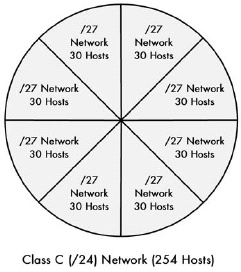
\includegraphics[width=.4\textwidth]{images/conventional-subnetting.jpg}
   \caption
      [Class C (/24) network split into eight conventional subnets]
      {Class C (/24) network split into eight conventional subnets --
      With traditional subnetting, all subnets must be the same size, which creates problems when there are some subnets that are much larger than others.
      Contrast this with \vref{fig:vlsm}.}
   \label{fig:conventional-subnetting}
\end{figure}



\subsection{The solution: variable-length subnet masking}

The solution is an enhancement to the basic subnet addressing scheme called \emph{variable-length subnet masking} (VLSM).
The idea is that you subnet the network and then subnet the subnets just the way you originally subnetted the network.
In fact, you can do this multiple times, creating subnets of subnets of subnets, as many times as you need
(subject to how many bits you have in the host ID of your address block).

It is possible to choose to apply this multiple-level splitting to only
some of the subnets, thereby allowing you to selectively cut the IP address pie so that some of the slices are bigger than others.
This means that the company in the previous example could create six subnets to match the needs of its networks, as shown in \cref{fig:vlsm}.


\begin{figure}
   \centering
   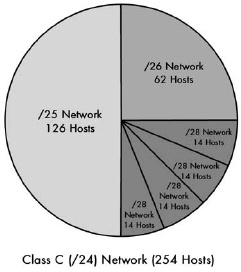
\includegraphics[width=.4\textwidth]{images/vlsm.jpg}
   \caption
      [Class C (/24) network split using VLSM]
      {Class C (/24) network split using VLSM -- 
      Using VLSM, an organization can divide its IP network multiple times to create subnets that match the size requirements of its physical networks much better.
      Contrast this with \cref{fig:conventional-subnetting}.}
   \label{fig:vlsm}
\end{figure}


\begin{keyconcept}
\emph{Variable-length subnet masking} (VLSM) is a technique for which subnetting is performed multiple times in iteration to allow a
network to be divided into a hierarchy of subnetworks that vary in size.
This allows an organization to better match the size of its subnets to the requirements of its networks.
\end{keyconcept}


\subsection{Multiple-level subnetting using VLSM}

VLSM subnetting is done the same way as regular subnetting; it just involves extra levels of subnetting hierarchy.
To implement it, you first subnet the network into large subnets and then further break down one or more of the subnets as required.
You add bits to the subnet mask for each of the sub-subnets and sub-sub-subnets to reflect their smaller size.

In VLSM, the slash notation of classless addressing is commonly used instead of binary subnet masks (it works very much like CIDR), so that's what I will use.

\begin{note}
If you're feeling a bit uncomfortable with how subnetting works, consider reading the chapter on practical subnetting
(\cref{chap:kozierok-ch19}) before proceeding with the VLSM example that follows.
\end{note}

For example, consider the class C network, 201.45.222.0/24.
You do three subnettings as follows (see \cref{fig:vlsm-example} for an illustration of the process).


\begin{figure}
   \centering
   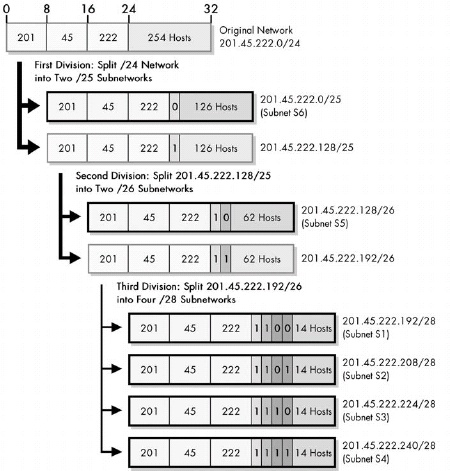
\includegraphics[width=.9\textwidth]{images/vlsm-example.jpg}
   \caption
      [VLSM example]
      {VLSM example -- 
      This diagram illustrates the example described in the text, of a class C (/24) network divided using three hierarchical levels.
      It is first divided into two subnets; one subnet is divided into two sub-subnets; and one sub-subnet is divided into four sub-sub-subnets.
      The resulting six subnets, shown with thick black borders, have a maximum capacity of 126, 62, 14, 14, 14, and 14 hosts.}
   \label{fig:vlsm-example}
\end{figure}


\begin{itemize}
\item
  You first do an initial subnetting by using one bit for the subnet ID,
  leaving you seven bits for the host ID and two subnets:
  201.45.222.0/25 and 201.45.222.128/25. Each of these can have a
  maximum of 126 hosts. You set aside the first of these for subnet S6
  and its 100 hosts.
\item
  You take the second subnet, 201.45.222.128/25, and subnet it further
  into two sub-subnets by taking one bit from the seven bits left in the
  host ID. This gives you the sub-subnets 201.45.222.128/26 and
  201.45.222.192/26, each of which can have 62 hosts. You set aside the
  first of these for subnet S5 and its 50 hosts.
\item
  You take the second sub-subnet, 201.45.222.192/26, and subnet it
  further into four sub-sub-subnets. You take two bits from the six that
  are left in the host ID, which gives you four sub-sub-subnets that
  each can have a maximum of 14 hosts. These are used for S1, S2, S3,
  and S4.
\end{itemize}

Although I've chosen these numbers so that they work out perfectly, you
should get the picture. VLSM greatly improves both the flexibility and
the efficiency of subnetting.


\begin{note}
In order to use VLSM, routers that support VLSM-capable routing protocols must be employed.
VLSM also requires more care in how routing tables are constructed to ensure that there is no ambiguity in how to interpret an address in the network.
\end{note}

As I mentioned earlier, VLSM is similar in concept to the way CIDR is performed.
The difference between VLSM and CIDR is primarily one of focus.
VLSM deals with subnets of a single network in a private organization.
CIDR takes the concept you just saw in VLSM to the Internet as a whole by changing how organizational networks are allocated,
replacing the single-level classful hierarchy with a multiple-layer hierarchy.
